\chapter{Problemanalyse und Anforderungsdefinition}
\label{cha:pua}

\emph{» Das Spiel ist die höchste Form der Forschung. «} \\
(Albert Einstein) \\

In diesem Kapitel werden folgende Aspekte behandelt: genauere Analyse der Aufgabenstellung, theoretische Anwendung der verschiedenen Lösungsansätze aus dem Grundlagenkapitel auf die beiden Strategiespiele Revesi und Tic Tac Toe, Einführung der Agentenmodelle, Beschreibung zweier bedeutender geschichtlicher Entwicklungen bezüglich dem lernen von Spielstrategien und definieren der Softwareziele in Anforderungen.

\section{Die Problematik}
Das Thema der Arbeit ist Untersuchung der Lernfähigkeit verschiedener Verfahren am Beispiel von Computerspielen. Bevor die Lernfähigkeit der Verfahren untersucht werden kann, müssen wir die Computerspiele festlegen und analysieren. Wie bereits erwähnt werden wir die Lernfähigkeit der Verfahren am Beispiel der Strategiespiele Reversi und Tic Tac Toe untersuchen (siehe Abbildung \ref{fig:reversi_und_tictactoe}). Eine genaue Beschreibung der Spielregeln, der Siegesbedingungen und möglicher Strategien bezüglich Heuristiken, wird in Kapitel \ref{cha:Modellierung und Entwurf} Modellierung und Entwurf erfolgen. Die zentrale Frage ist: wie kann ein Programm lernen ein Computerspiel erfolgreich zu spielen? \\

\begin{figure}[!htbp]
  \centering
  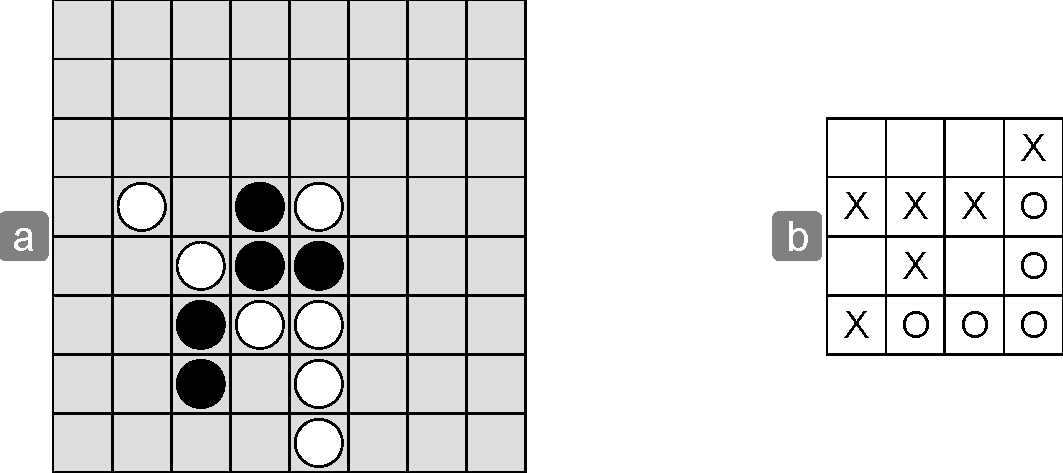
\includegraphics[scale = 0.8]{inhalt/abbildungen/reversi_und_tictactoe.pdf}
  \caption{Spielsituationen (Spielzustände oder Stellungen) die während einer Partie (a) Reversi oder (b) Tic Tac Toe auftreten können.}
  \label{fig:reversi_und_tictactoe}
\end{figure} 

\paragraph{Die Spieltheorie} aus Abschnitt \ref{sec:Spiele mit Gegner} liefert gleich mehrere Ansätze diese Frage zu beantworten. Die kombinatorische Suche (Abschnitt \ref{subsec:Minimax} Minimax) probiert einfach alle Möglichkeiten aus und liefert die beste gefundene Möglichkeit zurück. Die reine kombinatorische Minimax Suche ist praktisch jedoch nicht anwendbar, da, wie bereits im Abschnitt Minimax beschrieben wurde, die Anzahl der Kombinationsmöglichkeiten mit der Komplexität des Ausgangsproblems exponentiell ansteigt. \\

Selbst mit einer Kürzung von ganzen Unterbäumen des Suchbaums, ist die Rechenzeit für realistische Probleme nicht handhabbar (siehe Abschnitt \ref{subsec:Alpha-Beta-Kürzung} Alpha-Beta-Kürzung). Das Kürzen des Suchbaums kann unter Umständen mit einer iterativ vertiefenden Tiefensuche verbessert werden (siehe Abschnitt \ref{subsec:Iterativ vertiefende Tiefensuche} Iterativ vertiefende Tiefensuche). Die iterativ vertiefende Suche könnte Züge, z.B. in einer Tiefe von 2, sortieren. Vielversprechende Spielzüge könnten zu erst ausprobiert werden und das Alpha-Beta Verfahren könnte einen größeren Teil des Suchbaums kürzen. \\

Eine weitere Möglichkeit die Suche nach dem optimalen Spielzug in jeder Spielsituation zu verbessern, ist das Vermeiden von Übergängen. Ein Übergang oder Transition ist ein Spielzustand der mehrfach, an verschiedenen Stellen, in einem Suchbaum auftreten kann. Übergangstabellen und Transitions sind ausführlich in Abschnitt \ref{subsec:Übergangstabellen} Übergangstabellen erläutert. Eine Vermeidung dieser Übergänge könnte eine weitere Rechenzeitverringerung bewirken. \\

Die Heuristik oder Bewertungsfunktion ist wohl der wichtigste Leistungsfaktor aus den Verfahren der Spieltheorie (siehe Abschnitt \ref{subsec:Heuristik} Heuristik). Eine Heuristik kann jeden Knoten des Suchbaums bewerten (Nutzwert) und nicht nur die Blätter. Dies ermöglicht es die Suche nach einer bestimmten Zeitspanne oder iterierten Tiefe abzubrechen und den Spielzustand mit der besten Bewertung zurück zu geben. \\

Die Vorteile einer Heuristik sind die Limitierung der Zeit, die für eine Suche benötigt wird und dass das bisher beste gefundene Ergebnis zurück gegeben wird. Der große Nachteil einer Bewertungsfunktion ist, ein ermittelter Nutzwert für einen Spielzustand kann falsch sein. Die Qualität einer Heuristik ist also ausschlaggebend für die Spielstärke des Programms. Heuristiken sind zudem stark abhängig von ihrer Spielgrundlage, d.h. sowohl Reversi als auch Tic Tac Toe benötigen eigene Heuristiken, die individuell den Nutzen der Stellungen bewerten. \\

\begin{figure}[!htbp]
  \centering
  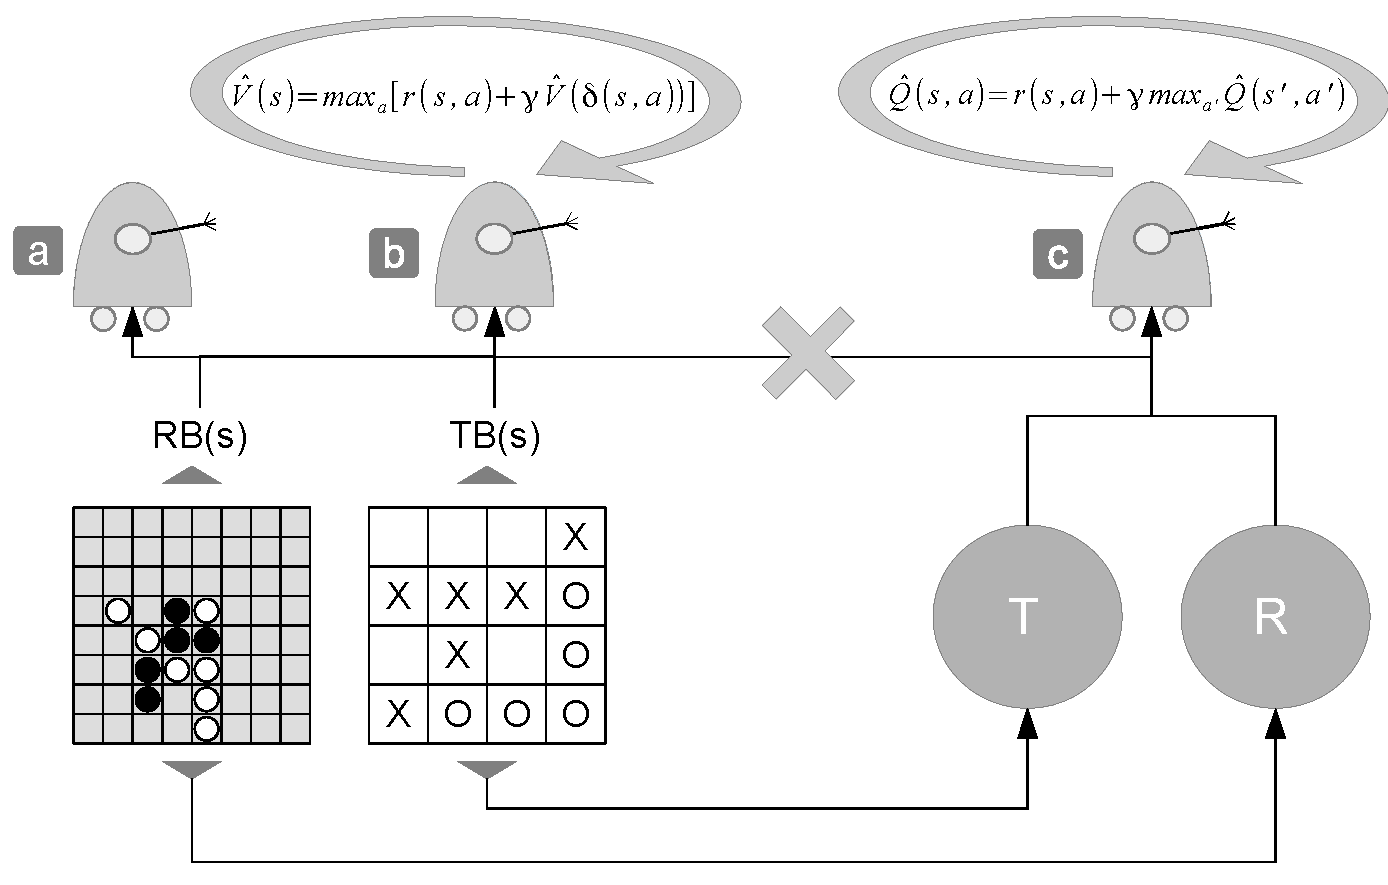
\includegraphics[scale = 0.6]{inhalt/abbildungen/drei_agenten.pdf}
  \caption{Die Projektproblematik.}
  \label{fig:drei_agenten}
\end{figure} 

\paragraph{Die drei Agenten} aus Abbildung \ref{fig:drei_agenten} repräsentieren drei Programme, die mit unterschiedlichen Verfahren, die selbe Aufgabe lösen. Die Aufgabe lautet: für jeden Spielzustand der Strategiespiele Reversi und Tic Tac Toe sollen die Agenten (a), (b) und (c) einen optimalen Spielzug (eine Aktion) vorschlagen, d.h. die Agenten müssen eine optimale Strategie anwenden. Eine optimale Strategie verwendet für jeden Möglichen Spielzustand immer den bestmöglichen Spielzug. \\

Agent (a) ist ein nicht lernender Agent, der Verfahren aus der Spieltheorie anwendet und dem die Bewertungsfunkionen RB(s) und TB(s) zur Verfügung stehen. RB(s) ist die Reversi Bewertungsfunktion, mit einem Reversi Spielzustand s als Eingabeparameter. TB(s) ist die Tic Tac Toe Bewertungsfunktion, mit einem Tic Tac Toe Spielzustand s als Eingabeparameter. \\

Agent (b) ist ein lernender Agent, der dem Agenten (a) sehr ähnlich ist, mit dem Unterschied, dass er die Gewichtungen (Faktoren $a_x$) der Bewertungsfunktionen mittels Spielerfahrung lernt. Agent (b) spielt eine festgelegte Anzahl von Spielen z.B. gegen sich selbst und verwendet eine Aktualisierungsfunktion $\hat{V}(s,a)$. Diese Funktion wurde bereits in Abschnitt \ref{subsec:Wert-Iteration und Dynamische Programmierung} Wert-Iteration und Dynamische Programmierung behandelt. Zusammengefasst ist diese Funktion eine Iterationsvorschrift, die mit der Bellman-Rekursionsgleichung die Gewichtungen der Heuristik so lange anpasst, bis diese sich nicht weiter verändern lassen und gegen eine optimale Strategie konvergieren. \\

Agent (c) ist ein lernender Agent, der im Gegensatz zu den Agenten (a) und (b) über kein Modell der Spielwelt verfügt, also ist ihm nicht bekannt in welchen Spielzustand ihn seine Aktionen führen. Er erhält auch keine Bewertungsfunktionen RB(s) und TB(s) für Spielzustände s. Alles was der Agent erhält sind zwei Menge T und R. Menge T enthält alle möglichen Aktionen die der Agent in einer bestimmten Tic Tac Toe Spielsituation ausführen darf, äquivalent dazu enthält Menge R alle möglichen Aktionen die der Agent in einer bestimmten Reversi Spielsituation ausführen darf. Nach einer bestimmten Anzahl von Aktionen erhält der Agent verspätet unterschiedliche Belohnungen für einen Sieg, eine Niederlage oder ein Unentschieden des Spiels. Der Agent verwendet das Lernverfahren $\hat{Q}$(s, a) aus Abschnitt  \ref{subsec:Q-Lernen}, um eine optimale Strategie zu lernen. \\

Sind alle Agenten implementiert, können wir beginnen die Lernfähigkeit der Agenten zu vergleichen. Wie werden die beiden lernenden Agenten gegen den nicht lernenden Agenten abschneiden? Welcher Agent wird der, der am meisten gewinnt und welcher Agent wird am meisten Verlieren? Wie viel Zeit benötigen die Agenten für die Berechnung der optimalen Strategie für die beiden Strategiespiele (Training)? Diese Fragen werden in Kapitel \ref{Auswertung} Auswertung beantwortet.

\section{Existierende Softwarelösungen}
Wir werden in diesem Teilabschnitt kurz einige der bekanntesten Softwarelösungen vorstellen. Dabei konzentrieren wir uns besonders auf die Konzepte, die die Programmierer angewendet haben, um Starke Computergegner zu realisieren. Alle hier vorgestellten Programme haben folgendes gemeinsam: sie sind gegen sehr gut menschliche Spieler getestet worden und es sind Anwendungen für 2-Spieler Strategiespiele. Ein großer Unterschied ist, dass Samuels Damespiel deterministisch und TD Gammon nichtdeterministische Spiele als Programmgrundlage haben.

\subsection{Samuels Damespiel}
\label{subsec:Samuels Damespiel}
Arthur L. Samuel schrieb 1955 ein Programm, dass Dame spielen konnte und mit einem einfachen Lernverfahren seine Parameter verbessern konnte. Sein Programm hatte dabei jedoch Zugriff auf eine große Zahl von archivierten Spielen, bei denen jeder einzelne Zug von Experten bewertet war. Damit verbesserte das Programm seine Bewertungsfunktion. Um eine noch weitere Verbesserung zu erreichen, ließ Samuel dein Programm gegen sich selbst spielen. Das Credit Assignment löste er auf einfache Weise. Für jede einzelne Stellung während eines Spiels vergleicht er die Bewertung durch die Funktion B(s) mit der durch Alpha-Beta-Pruning berechneten Bewertung und verändert B(s) entsprechend. 1961 besiegte sein Dame-Programm den viertbesten Damespieler der USA. Mit dieser bahnbrechenden Arbeit war Samuel seiner Zeit um fast dreißig Jahre voraus \cite[120\psq]{Ertel}.

\subsection{TD-Gammon}
\label{subsec:TD-Gammon}
Das TD-Lernen zusammen mit einem Backpropagation-Netz mit 40 bis 80 verdeckten Neuronen wurde sehr erfolgreich angewendet in TD-Gammon, einem Programm zum Spielen von Backgammon, programmiert vom Entwickler Gerald Tesauro im Jahr 1992. Die einzige direkte Belohnung für das Programm ist das Ergebnis am Ende eines Spiels. Eine optimierte Version des Programms mit einer 2-Züge-Vorausschau wurde mit 1,5 Millionen Spielen gegen sich selbst trainiert. Es besiegte damit Weltklassespieler und spielt so gut wie die drei besten menschlichen Spieler \cite[304]{Ertel}.  

\paragraph{Sind Lernverfahren überhaupt Sinnvoll?}

\section{Anforderungen}
\label{sec:Anforderungen}
Die nachfolgend definierten Anforderungen bilden die Grundlage des zu programmierenden Prototypen. Sie legen fest welche Funktionalitäten der Prototyp anbieten sollte und somit definieren sie die zu realisierenden Softwareziele des Projekts. Die Fett gedruckten Wörter sind die Bezeichnungen der Anforderungen. Die Zahlen vor den Bezeichnungen sind die Identifikatoren und der anschließende Text ist eine genauere Beschreibung der Anforderungen. \\

\begin{enumerate}
\item \textbf{Programmieren des Strategiespiels Tic Tac Toe}: \\
Das Programm soll die Tic Tac Toe Regeln anwenden, die Spielzustände sinnvoll realisieren und für Menschen lesbar darstellen können, eine Funktion beinhalten die einen Spielzug nach den Regeln durchführt und den Spielzustand dementsprechend anpasst, ein 4x4 Spielbrett mit 16 Spielfeldern bereitstellen und kein 3x3 Spielbrett wie bei dem klassischen Tic Tac Toe, den Spielzustand zurück geben können und Funktionen anbieten die einen Sieger bzw. Verlierer ermittelt. Ein beliebiger Spielzustand ist eine Repräsentation einer beliebigen Spielsteinstellung die während eines Spiels auftritt, sie beinhaltet alle sich noch auf den Spielfeldern befindenden Spielsteine, deren genaue Positionen und die Zugehörigkeit der Spielsteine zu den einzelnen Spielern.

\item \textbf{Programmieren des Strategiespiels Reversi}: \\
Dieses Programm soll die gleichen Funktionalitäten anbieten wie das Tic Tac Toe Spiel, mit folgenden Ausnahmen: die Spielregeln sollen Reversi(Othello) Spielregeln sein und das Spielbrett besteht aus 8x8, also 64 Spielfeldern.
	
\item \textbf{Funktionstest der Strategiespiele}: \\
Die Funktionen der programmierten Strategiespiele aus 1. und 2. sollen mit Unittests überprüft werden, um die Korrektheit der Programmlogik sicherzustellen.
	
\item \textbf{Heuristiken für beide Strategiespiele entwerfen}: \\
Im Abschnitt \ref{subsec:Heuristik} Heuristik haben wir bereits eine Schach Bewertungsfunktion B(s) gesehen. Diese erhält einen Spielzustand s als Parameter und evaluiert diese Stellung hinsichtlich der in der Bewertungsfunktion enthaltenen Merkmale und den dazugehörigen Gewichtungen $a_x$. Für die beiden Strategiespiele aus Anforderung 1 und 2 sollen ebenfalls Heuristiken mit angepassten Merkmalen entworfen werden.
	
\item \textbf{Entwickeln eines Agenten ohne Lernen}: \\
Der Agent soll die Konzepte aus Abschnitt \ref{sec:Spiele mit Gegner} Spiele mit Gegner anwenden. Besonders die Alpha-Beta-Suche, eine 2-Halbzüge Vorausschau und eine feste Heuristik.  Dieser Agent bekommt eine Heuristik übergeben und es ist ihm nicht erlaubt diese zu verändern bzw. die Gewichtungen der Merkmale der Heuristik. Der Agent Spielt Tic Tac Toe und Reversi ohne Lernen aber mit einer festen Stellungsbewertungsfunktion (Heuristik).
	
\item \textbf{Entwickeln eines Agenten der Heuristiken lernen}: \\
Ein Agent der ebenfalls die Konzepte aus Abschnitt \ref{sec:Spiele mit Gegner} Spiele mit Gegner realisieren soll. Der Unterschied zwischen diesem Agenten und dem Agenten aus Anforderung 5 ist, dieser Agent lernt die Gewichtungen der Heuristik-Merkmale auf Basis von Erfahrung, die er beim Spielen des Strategiespiels erhält.
	
\item \textbf{Entwickeln eines Agenten der ohne zusätzliches Wissen lernt}: \\
Dieser Agent unterscheidet sich stark von den Agenten die in den Anforderungen 5 und 6 definiert wurden, denn ihm wird kein zusätzliches Wissen, in Form einer Heuristik, mitgeteilt. Er soll auch keinen Minimax- oder Alpha-Beta-Suchbaum erstellen und durchsuchen. Vielmehr verfügt der Agent über eine eigene Lernstrategie (siehe Abschnitt \ref{sec:Verstärkendes Lernen} Verstärkendes Lernen), die Aktionen auswählt bis ein Spielergebnis feststeht und dann die Auswahl der Aktionen je nach Spielergebnis anpasst. Erfahrung sammelt der Agent im Spiel gegen sich selbst.
	
\item \textbf{Auswerten der Agentenqualität}: \\
Die Agenten sollen gegeneinander Spielen und die Spielergebnisse sollen erfasst werden. Die Auswertung dieser Ergebnisse soll zeigen welcher Agent wie oft gegen welchen Agenten verloren, gewonnen oder unentschieden gespielt hat. 
\end{enumerate}
